\section{Methodology}
\label{methodology}

At a high level\todo{Is this sufficient as a chapter ``roadmap'', or should I
    include one explicitly? How would I do this without duplication?}, our
methodology follows the following steps:

\input{build/methodOverview}

\def\addTextEx{For example, \citetISTQB{} \multiAuthHelper{cite}
    \citep{GerrardAndThompson2002} as the original source
    for \ifnotpaper their \else its \fi definition of ``scalability'' (see
    \Cref{scal-test-rec}); we verified\ptq{} this by
    looking at this original source.}

\subsection{Sources}
\label{sources}
As there is no single authoritative source on software testing terminology,
we need to look at many sources to observe how this terminology is used in
practice. Since we are particularly interested in software engineering, we
start from the vocabulary document for systems and software engineering%
\qtodo{Better name for this?}
\citep{IEEE2017} and two versions of the \acf{swebok}---the newest
one \citep{SWEBOK2014} and one submitted for public review\footnote{
    \refHelper \citep{SWEBOK2024} has been published since we investigated
    these sources; if time permits, we will revisit this published version.
} \citep{SWEBOK2024}---as \suggSrcs{}\todo{
    These are further justified later; should I put pointers here?
}. To gather further sources, we then use a version of ``snowball sampling'',
which ``is commonly used to locate hidden populations \dots{} [via] referrals
from initially sampled respondents to other persons'' \citep{Johnson2014}. We
apply this concept to ``referrals'' between sources. \addTextEx{} We similarly
``snowball'' on terminology itself; when a term requires more investigation
(e.g., its definition is missing or unclear), we perform a
miniature literature review on this subset to ``fill in'' this missing
information (see \Cref{undef-terms}). If these additional sources provide more
information and are ``trustworthy'', we may then investigate them in their
entirety (as opposed to just the original subset of interest). We define a
source to be ``trustworthy'' if it:
\begin{enumerate}
    \item has gone through a peer-review process,
    \item is written by numerous, well-respected authors,
    \item is informed by many sources, and
    \item is accepted and used in the field of software.
\end{enumerate}

For ease of discussion and analysis, we group the complete set of sources into
``tiers'' based on their format, method of publication, and this metric of
``trustworthiness''. We therefore create the following tiers, given in order of
descending trustworthiness: established standards (\Cref{stds}), terminology
collections (\Cref{metas}), textbooks (\Cref{texts}), and papers and other
documents (\Cref{papers}). Note that most sources used to ``fill in'' missing
information are papers. A summary of how many sources comprise each tier is
given in \Cref{fig:sourceSummary}.

% Only top or bottom to comply with IEEE guidelines
\begin{figure}[bt!]
    \centering
    \begin{tikzpicture}
        \pie[sum=auto, after number=, text=legend, thick,
            scale=\ifnotpaper0.7\else0.5\fi,
            every label/.style={align=left, scale=0.7}]
        {\stdSources{3}/\stds{},
            \metaSources{3}/\metas{},
            \textSources{3}/\texts{},
            \paperSources{3}/\papers{}}
    \end{tikzpicture}
    \caption{Summary of how many sources comprise each source tier.}
    \label{fig:sourceSummary}
\end{figure}

\ifnotpaper\newpage\fi

\subsubsection{\stdSources{1}}
\label{stds}
% Colored \textcolor{green}{green}

These are documents written for the field of software engineering by reputable
standards bodies, namely ISO, the \acf{iec}, and IEEE. Their purpose is to
``encourage the use of systems and software engineering standards'' and
``collect and standardize terminology'' by ``provid[ing] definitions that are
rigorous, uncomplicated, and understandable by all concerned''
\citep[p.~viii]{IEEE2017}. For these reasons\todo{Is this clear enough?}, they
are the most trustworthy sources. However, this does not imply perfection, as we
identify \stdSmntcDiscBrkdwn{13} % is (should be!) equal to \stdSntxDiscBrkdwn{13}
discrepancies within these standards (see \Cref{tab:sntxDiscreps,tab:smntcDiscreps})!
Only standards for software development and testing are in scope for
this research (see \Cref{scope}). For example, ``the purpose of the
ISO/IEC/IEEE 29119 series is to define an internationally agreed set of
standards for software testing that can be used by any organization when
performing any form of software testing''\todo{Does this add anything of value?}
\ifnotpaper(\fi\citeyear[p.~vii]{IEEE2022}\ifnotpaper; similar in
\citeyear[p.~ix]{IEEE2016})\fi.
This tier is composed of \stdSources{2}\todo{I sorted these so IEEE sources
    came first, since they focus on engineering. Should I explain this minor
    note? sort them another way?}.

\subsubsection{\metaSources{1}}
\label{metas}
% Colored \textcolor{blue}{blue}

These are collections of software testing terminology built up from multiple
sources (such as the established standards outlined in \Cref{stds}) that are
made to be widely applicable. For example, the \acs{swebok} is ``proposed as a
suitable foundation for government licensing, for the regulation of software
engineers, and for the development of university curricula in software
engineering'' \citep[p.~xix]{KanerEtAl2011}. They are often written by a large
organization, such as the \acf{istqb}, but not always. We include
\citeauthor{Firesmith2015}'s\todo{Correct grammar?} taxonomy
\citeyearpar{Firesmith2015} because it presents relations between many test
approaches and \citeauthor{DoğanEtAl2014}'s
literature review \citeyearpar{DoğanEtAl2014} because it cites many
of sources from which we can ``snowball'' if desired (see \Cref{sources}).
This tier is composed of \metaSources{2}.

\subsubsection{\textSources{1}}
\label{texts}
% Colored \textcolor{Maroon}{maroon}

We consider textbooks to be more trustworthy than papers (see \Cref{papers})
because they are widely used as resources for teaching software engineering and
may be used as guides in industry.\todo{Ideas on how to remove passive voice?}
Although textbooks have smaller sets of
authors, they follow a formal review process before publication. Textbooks used
at McMaster University \citep{Patton2006,PetersAndPedrycz2000,vanVliet2000}
served as the original (albeit ad hoc and arbitrary) starting point of this
research, and we investigate other books as they arise. \addTextEx{}
This tier is composed of \textSources{2}.

\subsubsection{\paperSources{1}}
\label{papers}
% Colored black

The remaining documents all have much smaller sets of authors and are much less
widespread than those in higher source tiers. While most documents are
journal articles and conference papers, the following document types are also
present. Some of these are less than academic, but show how terms are used in
practice; we include them in this source tier for brevity\thesisissueref{89}:

\begin{itemize}
    \item Report \citep{Kam2008,Gerrard2000a,Gerrard2000b}
    \item Thesis \citep{Bas2024}
          % \item A less-formal classification \citep{KuļešovsEtAl2013}
    \item Website \citep{LambdaTest2024,Pandey2023}
    \item Booklet \citep{SPICE2022}
    \item \ifnotpaper \else ChatGPT \fi \citet{ChatGPT2024} (with its claims
          supported by \citet{RusEtAl2008})
\end{itemize}

The full set of sources that comprise this tier is \paperSources{2}.

% Moved here to display nicely in paper
\ifnotpaper\else
    % Only top or bottom to comply with IEEE guidelines
    \begin{table*}[t!]
        \ieeeCatsTable{}
    \end{table*}
\fi

\subsection{Terminology}

\def\rigidBlurb{While most information is presented explicitly in the sources
    we investigate, some appears more implicitly. This is a useful distinction
    to make, as implicit claims carry less weight than explicit ones. We call
    this property ``rigidity''}

This research is intended to describe the current state of software testing
literature. To reduce potential bias, we do not invent or add our own
classifications or kinds of relations. Instead, the notions of test approach
categories (\Cref{categories-observ}), synonyms (\Cref{syn-rels}), and
parent-child relations (\Cref{par-chd-rels}) presented here
arose\ptq{} naturally from the literature. We define them here for clarity
since we use them throughout this \ifnotpaper thesis\else paper\fi, even
though they are ``results'' of our research. \rigidBlurb{} and define it
in \Cref{rigidity}.

\subsubsection{Approach Categories}
\label{categories-observ}

While there are many ways to categorize software testing approaches, perhaps
the most widely used is the one given by \ifnotpaper\else \citeauthor{IEEE2022}
\fi \citet{IEEE2022}, where a test approach can be categorized as a test level,
test type, test technique, or test practice (see \Cref{tab:ieeeCats}).
The categories of ``level'' and ``type'' are particularly common; for example,
six non-IEEE sources also give unit testing, integration testing,
system testing, and acceptance testing as examples of test levels \ifnotpaper
    (\citealp[pp.~5\=/6 to 5\=/7]{SWEBOK2024}; \citealpISTQB{};
    \citealp[pp.~807--808]{Perry2006}; \citealp[pp.~443--445]{PetersAndPedrycz2000};
    \citealp[p.~218]{KuļešovsEtAl2013}\todo{OG Black, 2009};
    \citealp[pp.~9, 13]{Gerrard2000a})\else
    \cite[pp.~443--445]{PetersAndPedrycz2000}, \cite{ISTQB},
    \cite[pp.~5\=/6 to 5\=/7]{SWEBOK2024}, \cite[pp.~9, 13]{Gerrard2000a},
    \cite[pp.~807--808]{Perry2006}, \cite[p.~218]{KuļešovsEtAl2013}%
    \todo{OG Black, 2009}\fi, although they may use a different term for ``test
level'' (see \Cref{tab:ieeeCats}). Because of their widespread use and
their usefulness in dividing the domain of software testing into more
manageable subsets, these categories are used for now. These four subcategories
of test approaches can be loosely described by what they specify as
follows\thesisissueref{21}:
\begin{itemize}
    \item \textbf{Level}: What code is tested
    \item \textbf{Practice}: How the test is structured and executed
    \item \textbf{Technique}: How to derive inputs and/or outputs
    \item \textbf{Type}: Which software quality is evaluated
\end{itemize}
For example, boundary value analysis is a test technique since its inputs are
``the boundaries of equivalence partitions'' \ifnotpaper
    (\citealp[p.~2]{IEEE2022}; \citeyear[p.~1]{IEEE2021}; similar on p.~12 and
    in \citealpISTQB{})%
\else
    \cite[p.~2]{IEEE2022}, \cite[p.~1]{IEEE2021}%
\fi. Similarly, acceptance testing is a test level since its goal is to
``enable a user, customer, or other authorized entity to determine whether to
accept a system or component'' \ifnotpaper (\citealp[p.~5]{IEEE2017}; similar
    in \citeyear[p.~6]{IEEE2021}; \citealp[p.~344]{SakamotoEtAl2013})\else
    \cite[p.~5]{IEEE2017}\fi, which requires the system or component to be
developed and ready for testing.

While the vast majority of identified test approaches can be categorized
in this way, \ifnotpaper there seem to be some outliers. For example, \fi
we also note the potential significance of an ``artifact'' category%
\thesisissueref{44,119,39}, since some terms could refer to the application of
a test approach and/or the resulting document(s). Because of this, a test
approach being categorized as a category from \Cref{tab:ieeeCats}
\emph{and} an artifact is \emph{not} a discrepancy\thesisissueref{119}
(see \Cref{multiCats}). \ifnotpaper
    Additionally, ``test metrics'' were also identified\thesisissueref{21,22},
    but tracking them is out-of-scope, since they describe methods for
    \emph{evaluating} testing as opposed to methods for \emph{performing} it.
    The related test approaches that seek to maximize these metrics are instead
    captured as kinds of coverage-driven testing (see \Cref{cov-test}) and
    experience-based testing \citep[p.~34]{IEEE2022}.

    \afterpage{
        \begin{landscape}
            % Moved earlier to display nicely in paper
            \ieeeCatsTable{}
            \newpage
            % Omitted from paper for brevity
            \otherCatsTable{}
        \end{landscape}
    }
\fi
Excluding \ifnotpaper our proposed \else this \fi ``artifact'' category, the
categories given in \Cref{tab:ieeeCats} seem to be orthogonal. For
example, ``a test type can be performed at a single test level or across
several test levels''
\ifnotpaper
    (\citealp[p.~15]{IEEE2022}; \citeyear[p.~7]{IEEE2021})%
\else
    \cite[p.~15]{IEEE2022}, \cite[p.~7]{IEEE2021}%
\fi, and ``Keyword-Driven Testing [sic] can be applied at all testing levels
\dots{} and for various types of testing'' \citeyearpar[p.~4]{IEEE2016}.
This means that a specific test approach can be derived by combining multiple
test approaches from different categories; for example, formal reviews are a
combination of formal testing and reviews. \ifnotpaper The following examples
    are given in the literature; the two subapproaches for each are omitted
    for brevity as the name of the combination makes it clear what they are:

    \phantomsection{}\label{orth-test-exs}
    \begin{enumerate}
        \item Black box conformance testing \citep[p.~25]{JardEtAl1999}
              %   (combining black box and conformance testing)
              % Specification-based: Technique (IEEE, 2022, p. 22; 2021, p. 8; Washizaki, 2024, p. 5-10; Hamburg and Mogyorodi, 2024; Souza et al., 2017, p. 3; Firesmith, 2015, pp. 46-47; Sakamoto et al., 2013, p. 344; implied by IEEE, 2022, pp. 2-4, 6-9)
              % Conformance: Type (implied by its quality (IEEE, 2017, p. 92; OG PMBOK 5th ed.))
        \item Black-box integration testing \citep[pp.~345--346]{SakamotoEtAl2013}
              % Specification-based: Technique (IEEE, 2022, p. 22; 2021, p. 8; Washizaki, 2024, p. 5-10; Hamburg and Mogyorodi, 2024; Souza et al., 2017, p. 3; Firesmith, 2015, pp. 46-47; Sakamoto et al., 2013, p. 344; implied by IEEE, 2022, pp. 2-4, 6-9)
              % Integration: Level (IEEE, 2022, pp. 12, 20-22, 26-27; 2021, p. 6; Washizaki, 2024, p. 5-7; Hamburg and Mogyorodi, 2024; Sakamoto et al., 2013, p. 343; Peters and Pedrycz, 2000, Tab. 12.3; van Vliet, 2000, p. 438; implied by Barbosa et al., 2006, p. 3)
              %           OR Technique (implied by Sharma et al., 2021, pp. 601, 603, 605-606)
        \item Checklist-based reviews \citepISTQB{}
              % Checklist-based: Practice (IEEE, 2022, p. 34), Technique (Hamburg and Mogyorodi, 2024)
              % Reviews: Approach
        \item Closed-loop HiL verification \citep[p.~6]{PreußeEtAl2012}
              % Closed Loop: Technique?
              % HiL: Out of Scope (hardware)
        \item Closed-loop protection system testing \citep[p.~331]{ForsythEtAl2004}
              % Closed Loop: Technique?
              % System: Level (IEEE, 2022, pp. 12, 20-22, 26-27; 2021, p. 6; 2017, p. 467; 2016, p. 4; Washizaki, 2024, p. 5-7; Hamburg and Mogyorodi, 2024; Sakamoto et al., 2013, p. 343; Peters and Pedrycz, 2000, Tab. 12.3; van Vliet, 2000, p. 439; implied by Barbosa et al., 2006, p. 3; Gerrard, 2000a, p. 13)
        \item Endurance stability testing \citep[p.~55]{Firesmith2015}
              % Endurance: Type (IEEE, 2013, p. 2; implied by Firesmith, 2015, p. 55)
              %         OR Technique (IEEE, 2021, p. 38)
              % Stability: Type (implied by its quality (IEEE, 2017, p. 434; OG ISO/IEC, 2009) and Firesmith, 2015, p. 55)
        \item End-to-end functionality testing (\citealp[p.~20]{IEEE2021}; \citealp[Tab.~2]{Gerrard2000a})
              % End-to-end: Type (Hamburg and Mogyorodi, 2024)
              %          OR Technique (Firesmith, 2015, p. 47; Sharma et al., 2021, pp. 601, 603, 605-606)
              % Functionality: Type (implied by its quality (IEEE, 2017, p. 196); Firesmith, 2015, p. 53)
        \item Formal reviews \citepISTQB{}
              % Formal: Technique (inferred from informal testing)
              % Reviews: Approach
        \item Grey-box integration testing \citep[p.~344]{SakamotoEtAl2013}
              % Grey-Box: Technique (IEEE, 2021, p. 8; Firesmith, 2015, pp. 46, 48; Sakamoto et al., 2013, p. 344)
              % Integration: Level (IEEE, 2022, pp. 12, 20-22, 26-27; 2021, p. 6; Washizaki, 2024, p. 5-7; Hamburg and Mogyorodi, 2024; Sakamoto et al., 2013, p. 343; Peters and Pedrycz, 2000, Tab. 12.3; van Vliet, 2000, p. 438; implied by Barbosa et al., 2006, p. 3)
              %           OR Technique (implied by Sharma et al., 2021, pp. 601, 603, 605-606)
        \item Incremental integration testing \citep[p.~601, 603, 605--606]{SharmaEtAl2021}\todo{OG [19]}
              % Incremental: Practice?
              % Integration: Level (IEEE, 2022, pp. 12, 20-22, 26-27; 2021, p. 6; Washizaki, 2024, p. 5-7; Hamburg and Mogyorodi, 2024; Sakamoto et al., 2013, p. 343; Peters and Pedrycz, 2000, Tab. 12.3; van Vliet, 2000, p. 438; implied by Barbosa et al., 2006, p. 3)
              %           OR Technique (implied by Sharma et al., 2021, pp. 601, 603, 605-606)
        \item Informal reviews \citepISTQB{}
              % Informal: Technique (implied by Kam, 2008, p. 6)
              % Reviews: Approach
        \item Infrastructure compatibility testing \citep[p.~53]{Firesmith2015}
              % Infrastructure: Type (implied by Firesmith, 2015, p. 57)
              %              OR Level (implied by Gerrard, 2000a, p. 13; see \Cref{tab:ieeeCats})
              % Compatibility: Type (IEEE, 2022, pp. 3, 22; 2021, p. 37, Tab. A.1; 2013, p. 2; implied by its quality (ISO/IEC, 2023a); Firesmith, 2015, p. 53)
        \item Invariant-based automatic testing \citep[pp.~184--185, Tab.~21]{DoğanEtAl2014},
              including for ``AJAX user interfaces'' \citetext{p.~191}
              % Assertion Checking: Practice?
              % Automated: Practice (IEEE, 2022, pp. 20, 22)
              %         OR Technique (implied by p. 35)
        \item Legacy system integration (testing) \citep[Tab.~2]{Gerrard2000a}
              % Legacy: Approach
              % System Integration: Level (IEEE, 2022, pp. 12, 22; 2021, p. 6; Hamburg and Mogyorodi, 2024)
        \item Manual procedure testing \citep[p.~47]{Firesmith2015}
              % Manual: Practice (IEEE, 2022, p. 22)
              %      OR Technique (implied by p. 35)
              % Procedure: Type (IEEE, 2022, pp. 7, 22; 2021, p. 39, Tab. A.1; 2017, p. 337; OG IEEE, 2013)
              %         OR Technique (implied by Firesmith, 2015, p. 47)
        \item Manual security audits \citep[p.~28]{Gerrard2000b}
              % Manual: Practice (IEEE, 2022, p. 22)
              %      OR Technique (implied by p. 35)
              % Security Audits: Technique (IEEE, 2021, p. 40)
              %               OR Type (inferred from security testing)
        \item Model-based GUI testing (\citealp[Tab.~1]{DoğanEtAl2014}; implied by \citealp[p.~356]{SakamotoEtAl2013})
              % Model-based: Practice (IEEE, 2022, p. 22; 2021, p. viii)
              %           OR Technique (Engström and Petersen, 2015, pp. 1-2; Kam, 2008, p. 4; implied by IEEE, 2022, p. 32; 2021, p. 7; 2017, p. 469)
              % GUI: Approach
        \item Model-based web application testing (implied by \citealp[p.~356]{SakamotoEtAl2013})
              % Model-based: Practice (IEEE, 2022, p. 22; 2021, p. viii)
              %           OR Technique (Engström and Petersen, 2015, pp. 1-2; Kam, 2008, p. 4; implied by IEEE, 2022, p. 32; 2021, p. 7; 2017, p. 469)
              % Web Application: Approach
        \item Non-functional search-based testing \citep[Tab.~1]{DoğanEtAl2014}
              % Non-functional: Approach
              % Search-based: Technique (Engström and Petersen, 2015, pp. 1-2)
        \item Offline MBT \citepISTQB{}
              % Offline: Practice?
              % Model-based: Practice (IEEE, 2022, p. 22; 2021, p. viii)
              %           OR Technique (Engström and Petersen, 2015, pp. 1-2; Kam, 2008, p. 4; implied by IEEE, 2022, p. 32; 2021, p. 7; 2017, p. 469)
        \item Online MBT \citepISTQB{}
              % Online: Practice?
              % Model-based: Practice (IEEE, 2022, p. 22; 2021, p. viii)
              %           OR Technique (Engström and Petersen, 2015, pp. 1-2; Kam, 2008, p. 4; implied by IEEE, 2022, p. 32; 2021, p. 7; 2017, p. 469)
        \item Role-based reviews \citepISTQB{}
              % Role-based: Practice?
              % Reviews: Approach
        \item Scenario walkthroughs \citep[Fig.~4]{Gerrard2000a}
              % Scenario: Technique (IEEE, 2022, pp. 9, 22; 2021, pp. 5, 8, 20, Fig. 2; 2017, p. 400; OG 2013; Washizaki, 2024, p. 5-12; Firesmith, 2015, p. 47; Sangwan and LaPlante, 2006, p. 26)
              % Walkthroughs: Technique (IEEE, 2017, p. 508)
        \item Scenario-based reviews \citepISTQB{}
              % Scenario-based: Approach
              % Reviews: Approach
        \item Security attacks \citepISTQB{}
              % Security: Type (IEEE, 2022, pp. 9, 22, 26-27; 2021, pp. 7, 40, Tab. A.1; 2017, p. 405; OG 2013; implied by its quality (ISO/IEC, 2023a; Washizaki, 2024, p. 13-4); Firesmith, 2015, p. 53)
              % Attacks: Practice (IEEE, 2022, p. 34)
              %       OR Technique (implied by Hamburg and Mogyorodi, 2024)
        \item Security audits (\citealp[p.~40]{IEEE2021}; \citealp[p.~28]{Gerrard2000b})
              % Security: Type (IEEE, 2022, pp. 9, 22, 26-27; 2021, pp. 7, 40, Tab. A.1; 2017, p. 405; OG 2013; implied by its quality (ISO/IEC, 2023a; Washizaki, 2024, p. 13-4); Firesmith, 2015, p. 53)
              % Audits: Practice?
        \item Statistical web testing \citep[p.~185]{DoğanEtAl2014}
              % Statistical: Technique (Kam, 2008, pp. 23, 48)      
              % Web Application: Approach
        \item Usability test script(ing) \citepISTQB{}
              % Usability: Type (IEEE, 2022, pp. 22, 26-27; 2021, pp. 7, 40, Tab. A.1; implied by its quality; Firesmith, 2015, p. 53)
              % Scripted: Practice (IEEE, 2022, pp. 20, 22; implied by p. 33)
        \item Web application regression testing \cite[Tab.~21]{DoğanEtAl2014}
              % Web Application: Approach
              % Regression: Technique (implied by IEEE, 2022, p. 35)
              %          OR Level (implied by Barbosa et al., 2006, p. 3)
        \item White-box unit testing \citep[pp.~345--346]{SakamotoEtAl2013}
              % Structure-based: Technique (IEEE, 2022, p. 22; 2021, p. 8; Washizaki, 2024, pp. 5-10, 5-13; Hamburg and Mogyorodi, 2024; Firesmith, 2015, pp. 46, 49; Sakamoto et al., 2013, p. 344; implied by IEEE, 2022, pp. 2, 4, 6, 9; Barbosa et al., 2006, p. 3)
              % Unit: Level (IEEE, 2022, pp. 12, 20-22, 26-27; 2021, p. 6; 2017, p. 467; 2016, p. 4; Washizaki, 2024, p. 5-6; Hamburg and Mogyorodi, 2024; Sakamoto et al., 2013, p. 343; Peters and Pedrycz, 2000, Tab. 12.3; van Vliet, 2000, p. 438; implied by Barbosa et al., 2006, p. 3)
              %    OR Technique (implied by Engström and Petersen, 2015, pp. 1-2)
    \end{enumerate}
    The subapproaches of the ``compound'' approaches given above are all from
    separate categories, when the following exceptional cases are considered:
    \begin{enumerate}
        \item \textbf{At least one subapproach is categorized inconsistently.}
              When a subapproach has more than one category (see \Cref{multiCats}),
              it is unclear which one should be used to assess orthogonality.
        \item \textbf{At least one subapproach's category is inferred.} When the category
              of a test approach is not given by the literature but is inferred
              from related context (see \Cref{infers}), it is unclear if it can
              be used to assess orthogonality.
        \item \textbf{At least one subapproach is only categorized as an approach.}
              Since ``approach'' is a catch-all categorization, it does not
              need to be orthogonal to its subcategories.
        \item \textbf{A subapproach is explicitly based on another in the same
                  category.} An example of this is stability testing, which
              tests a ``property that an object has with respect to a given
              failure mode if it cannot exhibit that failure mode''
              \citep[p.~434\todo{OG ISO/IEC, 2009}]{IEEE2017}. This notion of
              ``property'' is similar to that of ``quality'' that the test type
              category is built on, so it is acceptable that is implied to be
              a test type by its quality \citep[p.~434]{IEEE2017}%
              \todo{OG ISO/IEC, 2009} and by \citet[p.~55]{Firesmith2015}.
    \end{enumerate}
\fi

One important side effect of the particularity of these terms is that they can
be ``overloaded''; for example, someone could reasonably yet imprecisely use
any of these four categories as a synonym for ``approach''. Even the prompt in
\ifnotpaper \citep[emphasis added]{ChatGPT2024} \else \cite{ChatGPT2024} \fi was
imprecise, asking for the ``\emph{type} of software testing that focuses on
looking for bugs where others have already been found.'' Interestingly, ChatGPT
later ``corrected'' this by calling defect-based testing an approach!
Because of this, careful consideration needs to be given to discrepancies of
this nature. For example, \citet[p.~45\ifnotpaper, emphasis added\fi]{Kam2008}
defines interface testing as ``an integration \emph{test type} that is
concerned with testing \dots{} interfaces'', but since \ifnotpaper he \else it
\fi does not define ``test type'', this may not have special significance.
\ifnotpaper For this reason, these ``categorizations'' are marked with a
    question mark (?) and included in \Cref{tab:infMultiCats} instead of in
    \Cref{tab:multiCats}. In particular, other sources
    \citep[such as][]{SWEBOK2024,BarbosaEtAl2006} propose similar yet distinct
    categories that clash or overlap with these categories. These are given in
    \Cref{tab:otherCats} and may provide other perspectives when determining
    if \citep{IEEE2022}'s categorization is sufficient.

    The literature gives many other ways to categorize test approaches which
    are less-defined and seem to focus on specific categories from
    \Cref{tab:ieeeCats}. These are given in \Cref{tab:otherCategorizations} for
    completeness. The bases for these alternate categorizations, along with the
    example approaches listed, come from the source(s) indicated in the ``Test
    Basis'' column. When multiple names for a test basis are present, the union
    of their sources all list the examples given. By looking at a test basis
    and its corresponding examples, we can infer its ``Parent IEEE Category'':
    or the IEEE category from \Cref{tab:ieeeCats} it seems to subdivide. The
    sources provided in this column classify the example approaches given
    accordingly. For example, in the first row, \citet[pp.~4, 8]{IEEE2021} and
    \citet[p.~46]{Firesmith2015} both classify specification-based testing,
    structure-based testing, and grey-box testing as test techniques. A lack of
    source(s) in this column indicate that this category was inferred or that
    the example approaches were not categorized by the literature; additional
    context is sometimes provided in a footnote.

    \afterpage{
        \begin{landscape}
            \otherCategorizationsTable{}
        \end{landscape}
    }

    These categorizations may be used in tandem with or in place of those given
    in \Cref{tab:ieeeCats}, as these are more fine-grained. For example, some of
    these subsets, such as functional testing and structural testing, ``use
    different sources of information and have been shown to highlight different
    problems'' \citep[p.~5\=/16]{SWEBOK2024}. Likewise, some subsets may
    have ``conditions that make one approach more effective than the other'',
    such as deterministic testing and random testing \citetext{p.~5\=/16}.
    %\citep[p.~5\=/16]{SWEBOK2024}.
    Therefore, the existence of these classifications are not inherently wrong,
    as they may be useful for specific teams or in certain contexts.
    Unfortunately, even these categories are not used consistently (see
    \discrepref{manual-or-keyword,browser-static-and-dynamic})!

    Another way that the IEEE categories can be subdivided is by grouping related
    testing approaches into a ``class'' or ``family'' with ``commonalities and
    well-identified variabilities that can be
    instantiated'', where ``the commonalities are large and the variabilities
    smaller'' \citep{classFamilyDisc}. Examples of these are the classes of
    combinatorial \citep[p.~15]{IEEE2021} and data flow testing \citetext{p.~3} and
    the family of performance-related testing \perfAsFamily{}, and is implied for
    security testing, a test type that consists of ``a number of
    techniques\footnote{This may or may not be \distinctIEEE{technique}}''
    \cite[p.~40]{IEEE2021}. This is explored in more detail in
    \Cref{classFamilyDiscrep}. Note that ``there is a lot of overlap between
    different classes of testing'' \citep[p.~8]{Firesmith2015}, meaning that ``one
    category [of test techniques] might deal with combining two or more techniques''
    \citep[p.~5-10]{SWEBOK2024}. For example, ``performance, load and stress
    testing might considerably overlap in many areas'' \citep[p.~1187]{Moghadam2019}.
    A side effect of this is that it is difficult to ``untangle'' these classes;
    for example, take the following sentence: ``whitebox fuzzing extends dynamic
    test generation based on symbolic execution and constraint solving from unit
    testing to whole-application security testing''
    \citep[p.~23]{GodefroidAndLuchaup2011}! This is, in part, why research on
    software testing terminology is so vital.
\fi

\subsubsection{Synonym Relations}
\label{syn-rels}

The same approach often has many names. For example,
\emph{specification-based testing} is also called\todo{more in Umar2000}:
\begin{enumerate}
    \item Black-Box Testing
          \ifnotpaper
              (\citealp[p.~9]{IEEE2022}; \citeyear[p.~8]{IEEE2021};
              \citeyear[p.~431]{IEEE2017}; \citealp[p.~5\=/10]{SWEBOK2024};
              \citealpISTQB{}; \citealp[p.~46 (without hyphen)]{Firesmith2015};
              \citealp[p.~344]{SakamotoEtAl2013}; \citealp[p.~399]{vanVliet2000})
          \else
              \cite[p.~9]{IEEE2022}, \cite{ISTQB}, \cite[p.~431]{IEEE2017},
              \cite[p.~5\=/10]{SWEBOK2024}, \cite[p.~8]{IEEE2021},
              % \cite[p.~46 (without hyphen)]{Firesmith2015},
              \cite[p.~399]{vanVliet2000},
              \cite[p.~344]{SakamotoEtAl2013}
          \fi
    \item Closed-Box Testing
          \ifnotpaper
              (\citealp[p.~9]{IEEE2022}; \citeyear[p.~431]{IEEE2017})
          \else
              \cite[p.~9]{IEEE2022}, \cite[p.~431]{IEEE2017}
          \fi
    \item Functional Testing\footnote{This may be an outlier; see
              \Cref{spec-func-test}.}
          \ifnotpaper
              (\citealp[p.~196]{IEEE2017}; \citealp[p.~44]{Kam2008};
              \citealp[p.~399]{vanVliet2000}; implied by
              \citealp[p.~129]{IEEE2021}; \citeyear[p.~431]{IEEE2017})
          \else
              \cite[p.~196]{IEEE2017}, \cite[p.~399]{vanVliet2000},
              \cite[p.~44]{Kam2008} (implied by \cite[p.~431]{IEEE2017},
              \cite[p.~129]{IEEE2021})
          \fi
    \item Domain Testing \citep[p.~5\=/10]{SWEBOK2024}
    \item Specification-oriented Testing \citep[p.~440, Fig.~12.2]{PetersAndPedrycz2000}
    \item Input Domain-Based Testing (implied by \citealp[pp.~4\=/7 to
              4\=/8]{SWEBOK2014})
\end{enumerate}

These synonyms are the same as synonyms in natural language; while they may
emphasize different aspects or express mild variations, their core meaning
is nevertheless the same. Throughout our work, we use the terms
``specification-based testing'' and ``structure-based testing'' to articulate
the source of the information for designing test cases, but a team or project
also using grey-box testing may prefer the terms ``black-box'' and ``white-box
testing'' for consistency. Thus, synonyms are not inherently problematic,
although they can be (see \Cref{syns}).

Synonym relations are often given explicitly in the literature. For example,
\citet[p.~9]{IEEE2022} \multiAuthHelper{list} ``black-box testing'' and
``closed box testing'' beneath the glossary entry for ``specification-based
testing'', meaning they are synonyms. ``Black-box testing'' is likewise given
under ``functional testing'' in \citeyearpar[p.~196]{IEEE2017}, meaning it is
also a synonym for ``specification-based testing'' through transitivity%
\qtodo{Is this clear/correct? Should I explain this more?}.
However, these relations can also be less ``rigid'' (see \Cref{rigidity});
``functional testing'' is listed in a \emph{cf.} footnote to the glossary entry
for ``specification-based testing'' \citeyearpar[p.~431]{IEEE2017}, which
supports the previous claim but would not necessarily indicate a synonym
relation on its own.

Similarly, \citet[p.~5-10]{SWEBOK2024} says ``\emph{specification-based
    techniques} \dots{} [are] sometimes also called domain
testing techniques'' in the \acs{swebok} V4, from which the synonym of
``domain testing'' follows logically. However, its predecessor V3 only
\emph{implies} the more specific ``input domain-based testing'' as a synonym.
The section on test techniques says ``the classification of testing techniques
presented here is based on how tests are generated: from the software
engineer's intuition and experience, the specifications, the code structure
\dots'' \citep[p.~4\=/7]{SWEBOK2014}, and the first three subsections on the
following page are ``Based on the Software Engineer's Intuition and
Experience'', ``Input Domain-Based Techniques'', and ``Code-Based Techniques''
\citetext{p.~4\=/8}. The order of the introductory list lines up with these
sections, implying that ``input domain-based techniques'' are ``generated[]
from \dots{} the specifications'' (i.e., that input domain-based testing is the
same as specification-based testing). Furthermore, the examples of input
domain-based techniques given---equivalence partitioning, pairwise testing,
boundary-value analysis, and random testing---are all given as children%
\footnote{
    Pairwise testing is given as a child of combinatorial testing, which is
    itself a child of specification-based testing, by \ifnotpaper
        \citep[Fig.~2]{IEEE2021} and \citep[pp.~5\=/11 to 5\=/12]{SWEBOK2024}%
    \else
        \cite[pp.~5\=/11 to 5\=/12]{SWEBOK2024} and \cite[Fig.~2]{IEEE2021}%
    \fi, making it a ``grandchild'' of specification-based testing according to
    these sources.
} of specification-based testing \ifnotpaper
    (\citealp{IEEE2022}; \citeyear[Fig.~2]{IEEE2021}; \citealpISTQB{})\else
    \cite{IEEE2022,ISTQB}, \cite[Fig.~2]{IEEE2021}\fi; even V4 agrees with
this \citep[pp.~5\=/11 to 5\=/12]{SWEBOK2024}!

\subsubsection{Parent-Child Relations}
\label{par-chd-rels}
Many test approaches are multi-faceted and can be ``specialized'' into others;
for example, there are many subtypes of performance-related testing,
such as load testing and stress testing (see \Cref{perf-test-rec}). These
``specializations'' will be referred to as ``children'' or ``subapproaches''
of the multi-faceted ``parent''. This nomenclature also extends to other
categories (such as ``subtype''; see \Cref{categories-observ,tab:ieeeCats})
and software qualities (``subquality''\ifnotpaper; see \Cref{qual-test}\fi).
There are many reasons two approaches may have a parent-child relation, such as:
\qtodo{Should I add more? This would require me to go through my glossary and
    reverse engineer why I considered parent-child relations to be explicit. In
    hindsight, I should have recorded this as I went, and I'm not sure how
    worth it it would be to do now}
\begin{enumerate}
    \item \textbf{The parent approach is part of a mutually exclusive set.}
          It is often trivial to classify a test approach as a child of one of
          a set of other, mutually exclusive test approaches. For example,
          \citeauthor{IEEE2022} say that ``testing can take two forms: static
          and dynamic'' \citeyearpar[p.~17]{IEEE2022} and provide examples of
          subapproaches of static and dynamic testing \citetext{Fig.~1}.
          Likewise, \citeauthor{Gerrard2000a} says ``tests can be automated or
          manual'' \citeyearpar[p.~13]{Gerrard2000a} and gives subapproaches of
          automated and manual testing \ifnotpaper
              \citeyearpar[Tab.~2; ][Tab.~1]{Gerrard2000b}\else
              \citetext{Tab.~2}, \cite[Tab.~1]{Gerrard2000b}\fi.
    \item \textbf{One is ``stronger than'' or ``subsumes'' the other.} When
          comparing adequacy criteria that ``specif[y] requirements for
          testing'' \citep[p.~402]{vanVliet2000}, ``criterion X is stronger
          than criterion Y if, for all programs P and all test sets T,
          X-adequacy implies Y-adequacy'' \citetext{p.~432}. While this
          relation only ``compares the thoroughness of test techniques, not
          their ability to detect faults'' \citetext{p.~434}, it is sufficient
          to consider one a child of the other.
\end{enumerate}

\subsubsection{Rigidity}
\label{rigidity}

\def\impKeywordsCode{\seeSrcCode{55f4bf2}{helpers}{16}{32}}

A consequence of the use of natural language and the lack of standardization
is the considerable degree of nuance that can get lost when referring to
information sources. \rigidBlurb{} and capture it when citing sources. This
allows us to provide a more complete picture of the state of the literature;
for example, we can view implicit discrepancies separately in
\Cref{tab:sntxDiscreps,tab:smntcDiscreps}, since additional context may rectify
them. The following non-mutually exclusive reasons for information to be
considered ``implicit'' emerged, and the given keywords are used to identify
them \impKeywordsCode{}:

%% Maybe convert to \paragraph ?
\begin{enumerate}
    \item \textbf{The information is implied.} The implicit categorizations
          of ``test type'' by \citet[pp.~53--58]{Firesmith2015} (see
          \Cref{tab:multiCats\ifnotpaper,tab:infMultiCats\fi}) are an example
          of this. The given test approaches are not explicitly called ``test
          types'', as the term is used more loosely to refer to different kinds
          of testing---what should be called ``test approaches'' as per
          \Cref{tab:ieeeCats}. However, this set of test approaches are
          ``based on the associated quality characteristic and its associated
          quality attributes'' \citetext{p.~53}, implying that they are
          test types. Cases such as this are indicated by a question mark or
          one of the following keywords: ``implied'', ``inferred'', or
          ``likely''. \ifnotpaper \par
              Additionally, if a test approach in our glossary has a
              name ending in ``~(Testing)'' with a space, the word ``Testing''
              might not be part of its name \emph{or} it might not be a test
              approach at all! For example, the term ``legacy system
              integration'' is used \ifnotpaper by \citeauthor{Gerrard2000a}
                  (\citeyear[pp.~12--13, Tab.~2]{Gerrard2000a};
                  \citeyear[Tab.~1]{Gerrard2000b})\else in
                  \cite[pp.~12--13, Tab.~2]{Gerrard2000a},
                  \cite[Tab.~1]{Gerrard2000b}\fi, but the more accurate
              ``legacy system integration testing'' is used in
              \citeyearpar[pp.~30--31]{Gerrard2000b}. In other cases where a
              term is \emph{not} explicitly labelled as ``testing'', we add the
              suffix ``~(Testing)'' (when it makes sense to do so) and consider
              the test approach to be implied. \fi
    \item \textbf{The information is not universal.}
          \refHelper \citet[p.~372\ifnotpaper, emphasis added\fi]{IEEE2017}%
          \todo{OG ISO/IEC, 2014} \multiAuthHelper{define} ``regression
          testing'' as ``testing required to determine that a change to a
          system component has not adversely affected \emph{functionality,
              reliability or performance} and has not introduced additional
          defects''. While reliability testing, for example, is not
          \emph{always} a subset of regression testing (since it may be
          performed in other ways), it \emph{can be} accomplished by regression
          testing, so there is sometimes a parent-child relation (defined in
          \Cref{par-chd-rels}) between them. \ifnotpaper
          \citet[p.~5-8\ifnotpaper, emphasis added\fi]{SWEBOK2024} provides a
          similar list: ``regression testing \dots{} \emph{may} involve
          functional and non-functional testing, such as reliability,
          accessibility, usability, maintainability, conversion, migration, and
          compatibility testing.'' \fi Cases such as this are indicated by one
          of the following keywords: ``can be'', ``should be'', ``ideally'',
          ``usually'', ``most'', ``likely'', ``often'', or ``if''.
    \item \textbf{The information is conditional.}
          As a more specific case of information not being universal, sometimes
          prerequisities must be satisfied for information to apply. For
          example, branch condition combination testing is equivalent
          to (and is therefore a synonym of) exhaustive testing \emph{if} ``each
          subcondition is viewed as a single input'' \citep[p.~464]{PetersAndPedrycz2000}.
          Likewise, statement testing can be used for (and is therefore a child
          of) unit testing \emph{if} there are ``less than 5000 lines of code''
          \citetext{p.~481\todo{OG Miller et al., 1994}}. Cases such as this
          are indicated by the keyword ``can be'' or ``if''. \ifnotpaper
              \par This can also apply more abstractly at the taxonomy level,
              where a parent-child relation only makes sense if the parent test
              approach exists. This occurs when a source gives a relation
              between qualities but at least one of them does not have an
              explicit approach associated with it (although it may be derived;
              see \Cref{cov-test}). For example, \citet{ISO_IEC2023a} provides
              relations involving dependability and modifiability; these are
              tracked as qualities, not approaches, since only the qualities
              are described. Since the prerequisite of the relevant approach
              existing is \emph{not} satisfied, these relations are omitted
              from any generated graphs. \fi
    \item \textbf{The information is dubious.}
          This happens when there is reason to doubt the information provided.
          If a source claims one thing that is not true, related claims lose
          credibility. For example, the incorrect claim that ``white-box
          testing'', ``grey-box testing'', and ``black-box testing'' are
          synonyms for ``module testing'', ``integration testing'', and
          ``system testing'', respectively, \ifnotpaper (see
              \discrepref{dubious-syns}) \fi casts doubt on the claim that
          ``red-box testing'' is a synonym for ``acceptance testing''
          \citep[p.~18]{SneedAndGöschl2000}\todo{OG Hetzel88}\ifnotpaper\
              (see \discrepref{dubious-red-box-syn})\fi. Doubts such as this
          can also originate from other sources. \refHelper
          \citet[p.~48]{Kam2008} gives ``user scenario testing'' as a synonym
          of ``use case testing'', even though ``an actor [in use case testing]
          can be \dots{} another system'' \citep[p.~20]{IEEE2021}, which does
          not fit as well with the label ``user scenario testing''. However,
          since a system can be seen as a ``user'' of the test item, this
          synonym relation is treated as implicit instead of as an outright
          discrepancy. Cases such as this are indicated by a question mark or
          one of the following keywords: ``inferred'', ``should be'',
          ``ideally'', ``likely'', ``if'', or ``although''.
\end{enumerate}

Discrepancies based on implicit information are themselves implicit. These are
automatically detected when generating graphs and analyzing discrepancies
(see \ifnotpaper \Cref{graph-gen,discrep-analysis}, respectively\else
    \Cref{tools}\fi) by looking for the indicators of uncertainty mentioned
above \impKeywordsCode{}. These are used when creating
the glossaries to capture varying degrees of nuance, such as when a test
approach ``can be'' a child of another or is a synonym of another ``most of the
time'' but not always. \ifnotpaper As an example, \Cref{tab:parSyns} contains
    relations that are explicit, implicit, and both; implicit relations are
    marked by the phrase ``implied by''. \fi

\subsection{Procedure}
\label{procedure}

We track terminology used in the literature by building glossaries. The one
most central to our research is \ourApproachGlossary{}, where we give each
test approach its own row to
record its name and any given categories (see \Cref{categories-observ}),
synonyms (see \Cref{syn-rels}), parents (see \Cref{par-chd-rels}), and
definitions. If no category is given, the ``approach'' category is assigned
(with no accompanying citation) as a ``catch-all'' category. All other fields
may be left blank, but a lack of definition indicates that the approach should
be investigated further to see if its inclusion is meaningful (see
\Cref{undef-terms}). Any additional information from other sources is added to
or merged with the existing information in our glossary where appropriate.
This includes the generic ``approach'' category being replaced with a more
specific one, an additional synonym being mentioned, or another source
describing an already-documented parent-child relation. If any new information
contradicts existing information (or otherwise indicates something is wrong),
this is investigated and documented (see \Cref{discreps}), which may be done
in a separate document and/or in the glossary itself. Sometimes, new
information does not conflict with existing information, in which case the
clearest and most concise version is kept, or they are merged to paint a more
complete picture. Finally, we record any other notes, such as questions,
prerequisites, and other resources to investigate.

We use similar procedures to track software qualities \ifnotpaper (see
    \Cref{qual-test}) \fi and supplementary terminology (either shared by
multiple approaches or too complicated to explain inline) in separate
glossaries with a similar format. The name, definition, and synonym(s) of all
terms are tracked, as well as any precedence for a related test type for a
given software quality. We use heuristics to guide this process for all three
glossaries to increase confidence that all terms are identified, paying
special attention to the following when investigating a new source:

\begin{itemize}
    \item glossaries and lists of terms,
    \item testing-related terms (e.g., terms containing ``test(ing)'',
          \ifnotpaper ``review(s)'', ``audit(s)'', \fi
          ``validation'', or ``verification''),
    \item terms that had emerged as part of already-discovered
          testing approaches, \emph{especially} those that were ambiguous
          or prompted further discussion (e.g., terms containing
          ``performance'', ``recovery'', ``component'', ``bottom-up'',
          \ifnotpaper ``boundary'', \fi or ``configuration''), and
    \item terms that implied testing approaches%
          \ifnotpaper\footnote{
                  Since these methods for deriving test approaches only arose
                  as research progressed, some examples would have been missed
                  during the first pass(es) of resources investigated earlier
                  in the process. While reiterating over them would be ideal,
                  this may not be possible due to time constraints.
              } (see \Cref{derived-tests})\fi.
\end{itemize}
We apply these heuristics to most investigated sources, especially established
standards (see \Cref{stds}), in their entirety. Some sources, however, are only
partially investigated, such as those chosen for a specific area of
interest or based on a test approach that was determined to be out-of-scope.
These include the following sources as described in \Cref{undef-terms}:
\citep{ISO2022,ISO2015,Dominguez-PumarEtAl2020,PierreEtAl2017,
    TrudnowskiEtAl2017,YuEtAl2011,Tsui2007,Goralski1999}.

During the first pass of data collection, we investigate and record all
terminology related to software testing. Some of these terms are less
applicable to test case automation---our original motivation---%
\ifnotpaper(such as static testing; see \Cref{static-test}%
\thesisissueref{39})\ \fi%
or quite broad\ifnotpaper\ (such as attacks; see \Cref{attacks}%
    \thesisissueref{55})\fi, so they will be omitted during future analysis.
\ifnotpaper
    Others are so vague that they do not provide any new, meaningful
    information. For example, the ``systematic determination of the extent to
    which an entity meets its specified criteria'' \citep[p.~167]{IEEE2017} is
    certainly relevant to testing software; while this definition of
    ``evaluation'' may be meaningful when defining software testing generally,
    it does not define a new approach or procedure and applies much more
    broadly than just to testing. We decided\thesisissueref{39,44,28} that the
    following terms are too vague to merit tracking in our glossaries or
    analyzing further:
    \begin{itemize}
        \item \textbf{Evaluation:} the ``systematic determination of the extent
              to which an entity meets its specified criteria''
              \citep[p.~167]{IEEE2017}
        \item \textbf{Product Analysis:} the ``process of evaluating a product by
              manual or automated means to determine if the product has certain
              characteristics'' \citep[p.~343]{IEEE2017}
        \item \textbf{Quality Audit:} ``a structured, independent process to
              determine if project activities comply with organizational and
              project policies, processes, and procedures'' \citep[p.~361]{IEEE2017}
              \todo{OG PMBOK}
        \item \textbf{Software Product Evaluation:} a ``technical operation that
              consists of producing an assessment of one or more characteristics
              of a software product according to a specified procedure''
              \citep[p.~424]{IEEE2017}
    \end{itemize}

    \phantomsection{}\label{infers}
    Throughout this process, information can be inferred from ``surface-level''
    analysis that follows straightforwardly but isn't explicitly stated by any
    source. Examples of this are large scale integration testing and legacy
    system integration testing, described by \citeauthor{Gerrard2000a} in
    \citeyearpar[p.~30]{Gerrard2000b} and (\citeyear[Tab.~2]{Gerrard2000a};
    \citeyear[Tab.~1]{Gerrard2000b}), respectively. While he never explicitly
    says so, it can be inferred that these approaches are children of
    integration testing and system integration testing, respectively.
    Although these data do not come from the literature, they are documented
    for completeness; inferred discrepancies are given in \Cref{infer-discreps}
    and inferred relations, if any, are included in \recFigs{}.
\fi

\subsection{Undefined Terms}
\label{undef-terms}

The literature mentions many software testing terms without defining them.
While this includes test approaches, software qualities, and more general
software terms, we focus on the former as the main focus of our research.
In particular, many undefined test approaches are given by \citep{IEEE2022}
and \citep{Firesmith2015}. Once we exhaust the standards in \Cref{stds}, we
perform miniature literature reviews on these subsets to ``fill in'' the
missing definitions (along with any relations), essentially ``snowballing''
on these terms. This process uncovers even more approaches, although some are
out of scope, such as \acf{emsec} testing\ifnotpaper, \else\ and \fi
aspects of \acf{orthat} \ifnotpaper and loop testing \fi (see \Cref{hard-test})%
\ifnotpaper, and HTML testing (see \Cref{lang-test})\fi. The following terms
(and their respective related terms) were explored in the sources given:
\input{build/undefTerms}
Applying our procedure from \Cref{procedure} to these sources brings the number
of testing approaches from \the\TotalBefore{} to \the\TotalAfter{} and the
number of \emph{undefined} terms from \the\UndefBefore{} to \the\UndefAfter{}%
\ifnotpaper\ (see \Cref{fig:undefPies})\fi. This implies that about
\the\numexpr 100 - 100 * (\UndefAfter - \UndefBefore) / (\TotalAfter -
\TotalBefore)\relax\% of added test approaches are defined, which helps verify
that our procedure constructively uncovers new terminology.

\ifnotpaper
    \begin{figure*}
    \begin{subfigure}[c]{0.35\linewidth}
        \centering
        \begin{tikzpicture}[thick, scale=0.7, every label/.style={align=left, scale=0.7}]
            \pie[text=inside, sum=auto, color={blue!60, orange!60}]{
                {\the\numexpr \TotalBefore - \UndefBefore\relax}/,
                {\the\UndefBefore}/
            }
        \end{tikzpicture}
        \caption{The \the\TotalBefore{} approaches before investigating undefined terms.}
        \label{fig:undefPiesBefore}
    \end{subfigure}
    \hfill
    \begin{subfigure}[c]{0.35\linewidth}
        \centering
        \begin{tikzpicture}[thick, scale=0.7, every label/.style={align=left, scale=0.7}]
            \pie[text=inside, sum=auto, color={blue!60, orange!60}]{
                {\the\numexpr \TotalAfter - \UndefAfter\relax}/,
                {\the\UndefAfter}/
            }
        \end{tikzpicture}
        \caption{The \the\TotalAfter{} approaches after investigating undefined terms.}
        \label{fig:undefPiesAfter}
    \end{subfigure}
    \hfill
    \begin{subfigure}[c]{0.2\linewidth}
        \centering
        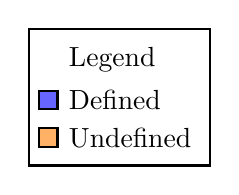
\begin{tikzpicture}
            \matrix [thick, draw=black] {
            \node[label=right:{Legend}] {}; \\
            \node[thick, shape=rectangle, draw=black, fill=blue!60,   label=right:{Defined}](0) {}; \\
            \node[thick, shape=rectangle, draw=black, fill=orange!60, label=right:{Undefined}](1) {}; \\
            };
        \end{tikzpicture}
    \end{subfigure}
    \caption{Breakdown of how many test approaches are undefined.}
    \label{fig:undefPies}
\end{figure*}

\fi

In addition to terms with missing definitions, some terms do not appear in
the literature at all! While most test approaches arise as a result of our
snowballing approach, we each have preexisting knowledge of what test
approaches exist (a form of experience-based testing, if you will%
\qtodo{Is this ``joke'' too distracting?}).
As an example, we are surprised that property-based testing is not mentioned
in any sources investigated, even using it as a target ``stopping point''
throughout this process\thesisissueref{57,81,88,125}\qtodo{I think these issue
    refs, along with some others may actually be worth keeping in our final
    thesis/paper; thoughts?}. Test approaches such as these that arise
independently of snowballing may serve as starting points for continuing
research if they are not mentioned by the literature. The following terms come
from previous knowledge, conversations with colleagues, research for other
projects, or ad hoc cursory research to see what other test approaches exist:
\ifnotpaper \begin{multicols}{2} \fi
        \begin{enumerate}
            \item Chaos engineering
            \item Chosen-ciphertext attacks
            \item Concolic testing
            \item Concurrent testing
            \item Destructive testing
            \item Dogfooding
            \item Implementation-based testing
            \item Interaction-based testing
            \item Lunchtime attacks\ifnotpaper%
                      \footnote{In previous meetings, Dr.~Smith mentioned
                          that with the number of test approaches that suggest
                          that people just like to label everything as
                          ``testing'', he would not be surprised if something
                          like ``Monday morning testing'' existed. While
                          independently researching chosen-ciphertext attacks
                          out of curiosity, this prediction of a time-based
                          test approach came true with ``lunchtime attacks''.}
                  \fi
            \item Parallel testing
            \item Property-based testing
            \item Pseudo-random bit testing
            \item Rubber duck testing
            \item Shadow testing
        \end{enumerate}
        \ifnotpaper \end{multicols} \fi
